\documentclass[11pt,letterpaper]{article}
\usepackage{macroshw}

\title{\begin{spacing}{1.2}Electrodynamics I\\HW 5\end{spacing}}
\author{Matthew Phelps}
\date{Due: April 21}

\begin{document}
\maketitle

\benum
% #1 --------------------------------------------------------------------------------------------------------------------------------------------------------------------------------------
  	\item 
	A constant electric current $I$ flows through an infinite cylinder non-magnetic conductor of radius $a$. Density of the electric 
	current inside a conductor is uniform. Determine the magnetic induction $\vect B(\vect r)$ and vector potential $\vect A(\vect r)$
	of the induced magnetic field. 
	\\
	\\
	First let's calculate the current density
	\[
		I = \int \vect J(\vect x)\cdot d\vect S = J(\pi a^2)
	\]
	thus
	\[
		\vect J = \frac{I}{\pi a^2}\vecth z\qquad (\rho\le a)
	\]
	where we have chosen the cylinder to be aligned along the $z$-axis for convenience. It will be beneficial to note the direction of the
	magnetic field inside and outside the cylinder by using the Biot-Savart law
	\[
		d\vect B = kI\frac{(d\vect l\times \vect x)}{|\vect x|^3}
	\]
	where $\vect x$ is the vector from an element of current length to an observation point. From this law we can see that behavior of the
	magnetic field from a straight cylinder of current must lie solely in the $\vecth \phi$ direction. As a problem in magnetostatics we work
	under the regime that the charge density does not change,
	\[
		\pdiff[\rho]{t} = 0
	\]
	and therefore
	\[
		\del\cdot\vect J = 0
	\]
	by the continuity equation. From the Biot-Savart law we may also derive the differential laws of the magnetic field:
	\be\label{1}
		\del\cdot \vect B = 0
	\ee
	and 
	\be\label{2}
		\del\times \vect B = \mu_0\vect J.
	\ee
	By integrating \eqref 2 we can find the magnetic field using Stokes law (the resulting equation is Amperes's law) 
	\[
		\int (\del\times\vect B)\cdot d\vect S = \mu_0 \int \vect J\cdot d\vect S
	\]
	\[
		\oint \vect B\cdot d\vect l = \mu_0 I_{enc}.
	\]
	Outside the cylinder the magnetic field points in the $\vecth \phi$ direction, so we choose a circular loop of radius $\rho$ and 
	solve for the magnetic field
	\[
		\vect B = \frac{\mu_0 I}{2\pi\rho}\vecth\phi		\quad(\rho\ge a).
	\]
	For points inside the cylinder the magnetic field can be seen to still point in the $\vecth \phi$ direction but now the enclosed current 
	becomes
	\[
		I_{enc} = \int_{\rho\le a} \vect J\cdot d\vect S = I\pfrac{\rho^2}{a^2}.
	\]
	Thus the magnetic field from Ampere's law is then
	\[
		\vect B = \frac{\mu_0 I}{2\pi}\frac{\rho}{a^2}\vecth \phi	\quad(\rho\le a).
	\]
	The magnetic field in total is
	\[
		\vect B = \begin{cases}\ds \frac{\mu_0 I}{2\pi}\frac{\rho}{a^2}\vecth\phi &\quad (\rho \le a)\\  \\\ds
				 \frac{\mu_0 I}{2\pi\rho}\vecth\phi&\quad(\rho \ge a)
				\end{cases}
	\]
	Since the divergence of $\vect B$ is zero the magnetic field can also be expressed in terms of an arbitrary vector potential
	\[
		\vect B = \del\times\vect A.
	\]
	The arbitrariness of such a vector potential comes from the fact that it defined up to the gradient of a scalar. In other words
	\[
		\del\times\vect A = \del\times(\vect A+\del\Psi)
	\]
	where $\Psi$ is any scalar function. For reasons that are not yet known, we will choose to constrain $\vect A$ to the Coulomb gauge
	defined as
	\[
		\del\cdot\vect A = 0.
	\]		
	From the Biot-Savart law, we know that $\vect A$ in the Coulomb gauge takes the form
	\[
		\vect A(\vect x)  = \frac{\mu_0}{4\pi}\int \frac{\vect J(\vect x')}{|\vect x-\vect x'|}d^3x' .
	\]
	To calculate what the vector potential is for a cylinder of infinite current, it is helpful to notice that $\vect A$ always lies in the same
	direction as $\vect J$. Thus $\vect A$ must have a component only in the $\vecth z$ direction
	\[
		\vect A = A\vecth z.
	\]
	In addition, we know that the curl of $\vect A$ must only have a component in the $\vecth \phi$ direction. 
	We can use this information to show that
	\be\label{3}
		A  = -\int B \, d\rho + f(\phi,z)
	\ee
	and
	\be\label{4}
		\frac{1}{\rho}\pdiff[A]{\phi}  = 0.
	\ee
	From the Coulomb gauge condition, we have in addition 
	\be\label{5}
		\pdiff[A]{z} = 0.
	\ee
	From \eqref 4 and \eqref 5 we see that 
	\[
		f(\phi,z) = C
	\]
	and thus
	\[
		A = -\int B\, d\rho + C.
	\]
	Solving for $A$ we find
	\[
		A = \begin{cases}\ds -\frac{\mu_0 I}{4\pi}\frac{\rho^2}{a^2}+C_1 &\quad(\rho \le a)\\ \\ \ds
			-\frac{\mu_0 I}{2\pi}\ln(\rho)+C_2 &\quad(\rho \ge a).
			\end{cases}
	\]
	While not strictly necessary, we can choose to make $A$ continuous at $\rho = a$ by a proper choice of constants
	\[
		 -\frac{\mu_0 I}{4\pi}+C_1 = -\frac{\mu_0 I}{2\pi}\ln(a)+C_2.
	\]
	A simple choice turns out to be one such that $A(a) = 0$
	\[
		-\frac{\mu_0 I}{4\pi}+C_1 = 0\quad\to\quad C_1 = \frac{\mu_0 I}{4\pi}
	\]
	and
	\[
		-\frac{\mu_0 I}{2\pi}\ln(a)+C_2\quad\to\quad C_2= \frac{\mu_0 I}{2\pi}\ln(a).
	\]
	Having solved the coefficients, the vector potential and magnetic field are
	\[
		\vect A = \begin{cases} \ds -\frac{\mu_0 I}{4\pi a^2}(\rho^2-a^2)\vecth z&\quad(\rho\le a)\\ \\ \ds
					-\frac{\mu_0 I}{2\pi}\ln\pfrac{\rho}{a}\vecth z&\quad(\rho\ge a)
				\end{cases}
	\]
	\[
		\vect B = \begin{cases}\ds \frac{\mu_0 I}{2\pi}\frac{\rho}{a^2}\vecth\phi &\quad (\rho \le a)\\  \\\ds
				 \frac{\mu_0 I}{2\pi\rho}\vecth\phi&\quad(\rho \ge a)
				\end{cases}
	\]
	\\
	\\
% #2 ------------------------------------------------------------------------------------------------------------------------------------------------------------------------------------
	\item
	A straight and infinitely long strip of width $a$ carries uniformly distributed electric current $I$. Calculate the magnetic 
	induction $\vect B(\vect r)$ and determine the asymptotic behavior of the magnetic field at large distances from the strip.
	\\
	\\
	We will take our infinite strip to have current running in the $\vecth z$  direction with strip width running from $-a/2\le x \le a/2$. By the 
	Biot Savart law, we know the magnetic field must be perpendicular to $\vecth z$ and thus it will only have components in the $x$-$y$ 
	plane. 
	\\
	\\
	A good starting point is that of the field due to an infinitely long straight wire with magnetic field
	\[
		\vect B = \frac{\mu_0 I}{2\pi |\vect r|}(\vecth z \times \vecth r).
	\]
	To find the magnetic field for a strip, we will need to integrate this magnetic field over a sum of infinitesimal wires. Let's denote the
	surface charge density as $\vect K = K\vecth z$ so that
	\[
		dI = K\,dx.
	\]
	The surface charge density can also be expressed in terms of the total strip length as
	\[
		K = \frac{I}{a}.
	\]
	The magnetic field at an observation point $P = (x,y)$ has the distance vector 
	\[
		\vect r = (x-x_0)\vecth x + y \vecth y.
	\]
	The direction of the magnetic field is then
	\[
		\vecth z \times \vecth r = \frac{-y\vecth x +(x-x_0)\vecth y}{|\vect r|}.
	\]
	Putting these results all together, we find the magnetic field at a point $P(x,y)$ is given as
	\[
		d\vect B = \frac{\mu_0 I}{2\pi a}\plr{\frac{-y\, dx_0}{(x-x_0)^2+y^2}}\vecth x +
		 \frac{\mu_0 I}{2\pi a} \plr{\frac{(x-x_0)\, dx_0}{(x-x_0)^2+y^2}}\vecth y.
	\]
	To find the total field, we integrate. Starting with the $x$ component of the magnetic field
	\[
		B_x = \frac{\mu_0 I}{2\pi a} \int_{-a/2}^{a/2} dx_0\, \frac{-y}{(x-x_0)^2+y^2}.
	\]
	With a change of variable
	\[
		u = \frac{x-x_0}{y},\quad dx_0 = -y\, du
	\]
	\ba
		B_x &= \frac{\mu_0 I}{2\pi a}\int_{\frac{x+a/2}{y}}^{\frac{x-a/2}{y}}
		\frac{du}{u^2+1}\\
		& = \frac{\mu_0 I}{2\pi a}\tan^{-1}(u)|_{\frac{x+a/2}{y}}^{\frac{x-a/2}{y}}\\
		& =  \frac{\mu_0 I}{2\pi a}\blr{\tan^{-1}\pfrac{x-a/2}{y}- \tan^{-1}\pfrac{x+a/2}{y}}
	\ea
	Now for the $y$ component (with a change of variable $u = x - x_0$)
	\ba
		B_y &= \frac{\mu_0 I}{2\pi a} \int_{x+a/2}^{x-a/2} du\, \frac{-u}{u^2+y^2}\\
		& = \frac{\mu_0 I}{2\pi a} \pfrac{-1}{2} \ln(u^2+y^2)|_{x+a/2}^{x-a/2}\\
		& = \frac{\mu_0 I}{4\pi a}\ln\blr{\frac{(x+a/2)^2+y^2}{(x-a/2)^2+y^2}}.
	\ea
	In total we have
	\ba
		\vect B(x,y) =& \frac{\mu_0 I}{2\pi a}\blr{\tan^{-1}\pfrac{x-a/2}{y}- \tan^{-1}\pfrac{x+a/2}{y}}\vecth x\\
		&+ \frac{\mu_0 I}{4\pi a}\ln\blr{\frac{(x+a/2)^2+y^2}{(x-a/2)^2+y^2}}\vecth y.
	\ea
	Here is a nice figure of the magnetic field in the $x$-$y$ plane produced by the strip. Notice that the magnetic field 
	looks that like of a single wire at distances far from the plate. 
	\\
		\begin{figure}[H]
			\centering
			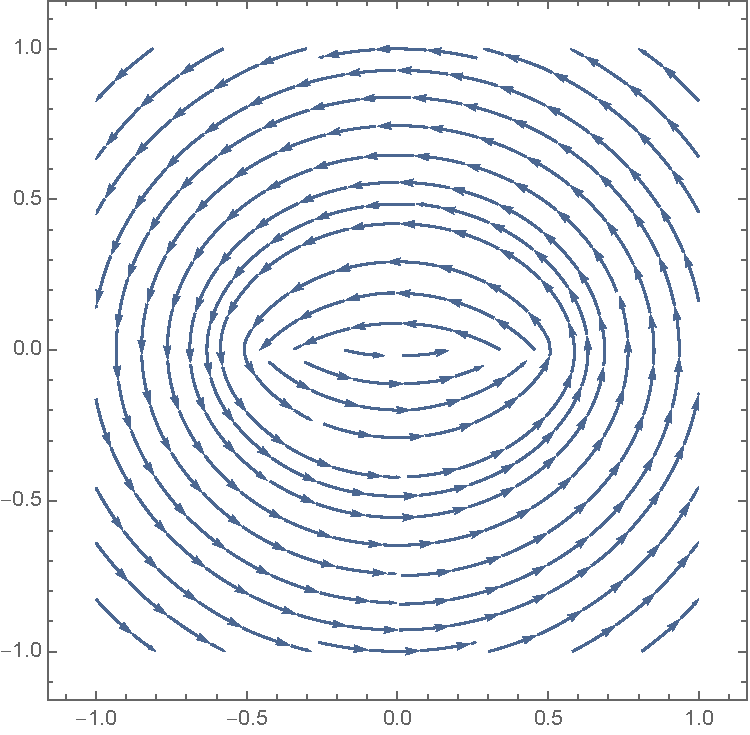
\includegraphics[width=100mm]{2_HW5.pdf}
		\end{figure}
	For the expansion of $B_x(x,y)$ for large $r$, we first write our terms as
	\[
		\tan^{-1}\plr{\frac{x}{y}-\frac{a/2}{y}}-\tan^{-1}\plr{\frac{x}{y}+\frac{a/2}{y}}.
	\]
	Using the taylor expansion
	\[
		f(x+h) = f(x)+hf'(x)+...
	\]
	the inverse tangent can be approximated for small $t$ as
	\[
		\tan^{-1}(s+t) = \tan^{-1}(s)+ \frac{t}{1+s^2}+...
	\]
	In the $\lim x,y\to \infty$ we note that $\frac{a/2}{y} \to 0$. If we work under the assumption that 
	\[
		\frac{x}{y} \gg \frac{a/2}{y} 
	\]
	then we can utilize the substitutions
	\[
		\frac{x}{y} = s,\quad \frac{a/2}{y} = t,
	\]
	such that $s\gg t$. We then form the expansion 
	\ba
		\tan^{-1}\plr{\frac{x}{y}-\frac{a/2}{y}} &\approx \tan^{-1}\pfrac{x}{y} -\pfrac{\frac{a/2}{y}}{1+\frac{x^2}{y^2}}\\
		& = \tan^{-1}\pfrac{x}{y}-\frac{ya/2}{x^2+y^2}.
	\ea
	Similarly for the other term we find
	\[
		\tan^{-1}\plr{\frac{x}{y}+\frac{a/2}{y}} \approx \tan^{-1}\pfrac{x}{y}+\frac{ya/2}{x^2+y^2}
	\]
	Subtracting the two from each other we form
	\[
		\tan^{-1}\plr{\frac{x}{y}-\frac{a/2}{y}}-\tan^{-1}\plr{\frac{x}{y}+\frac{a/2}{y}} \approx -\frac{ya}{x^2+y^2}.
	\]
	Thus for the $x$ component of the $B$ field we have
	\[
		B_x\approx -\frac{\mu_0 I}{2\pi}\pfrac{y}{x^2+y^2}.
	\]
	For the $B_y$ component we have the natural log term we need to expand.
	\ba
		&\ln[(x+a/2)^2+y^2]-\ln[(x-a/2)+y^2] \\
		=& \ln[x^2+y^2+ax+a^2/4] - \ln[x^2+y^2-ax+a^2/4].
	\ea
	For $s\gg t$ the first order Taylor expansion of the log goes as
	\[
		\ln(s+t) = \ln(s)+\frac{t}{s}+...
	\]
	This time we work under the assumption that $x^2+y^2 \gg ax+a^2/4$ such that we use the variables
	\[
		s = x^2+y^2,\quad h = ax+a^2/4.
	\]
	We then have the expansion
	\ba
		& \ln[x^2+y^2+ax+a^2/4] - \ln[x^2+y^2-ax+a^2/4] \\
		\approx& \ln(x^2+y^2) + \frac{ax+a^2/4}{x^2+y^2} - \ln(x^2+y^2) + \frac{ax-a^2/4}{x^2+y^2} \\
		 = &  \frac{2ax}{x^2+y^2}.
	\ea
	Thus the $y$ component of the magnetic field is
	\[
		B_y = \frac{\mu_0 I}{2\pi}\pfrac{x}{x^2+y^2}.
	\]
	Since we are restricting our attention to the $x$-$y$ plane here, we note that the unit vector in the $\vecth \phi$ direction
	can be substituted as
	\[
		\vecth \phi = -\sin\phi \vecth x+\cos\phi \vecth y.
	\]
	If we now make the appropriate substitutions
	\[
		x = r\cos\phi,\quad y = r\sin\phi,\quad r^2 = x^2+y^2
	\]
	we finally arrive at
	\[
		\vect B = \frac{\mu_0 I}{2\pi r}\vecth \phi
	\]
	which is precisely the magnetic field due to a single straight wire!  
	\\
% #3 ------------------------------------------------------------------------------------------------------------------------------------------------------------------------------------
	\item
	Two thin infinitely long parallel plates carry equal and opposite currents $I$. The width of each plate is $a$ and the distance
	between them is $b$. For each plate, determine the force $f$ per unit of length.
	\\
	\\
	The magnetic field found found in the last problem can be directly applied to the situation of two parallel plates. From the symmetry of the 
	system we can see that the forces in the $x$ direction are equal and opposite and thus we only need to look 
	at the $y$ component of the force. This can also be seen by a figure of the vector force field produced by the magnetic field of the plate 
	at the origin acting on a single wire with current in the $-\vecth z$ direction. 
	\\
		\begin{figure}[H]
			\centering
			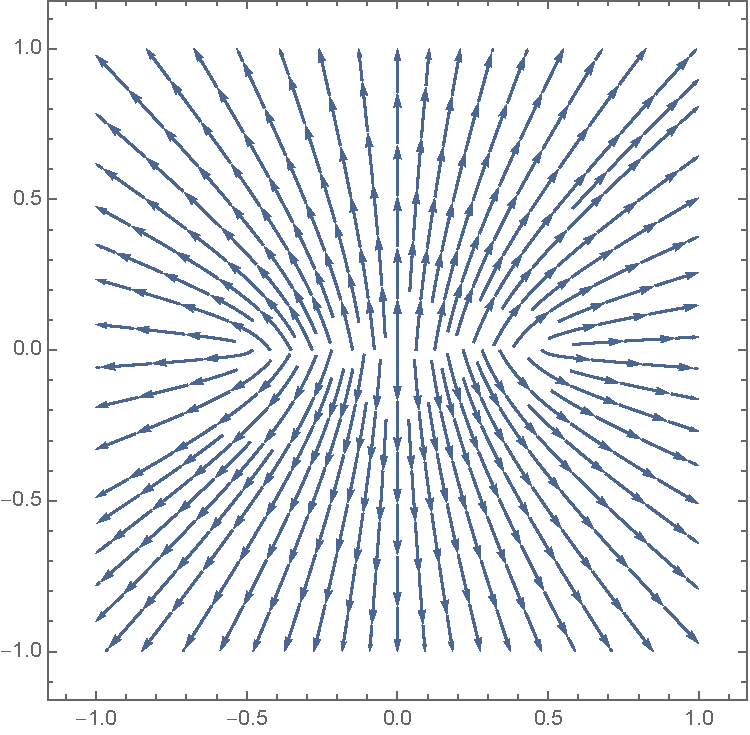
\includegraphics[width=100mm]{3_HW5.pdf}
		\end{figure}
	With one plate at the origin, we see that the force acting on the opposite plate is repulsive. 
	\\
	\\
	To calculate the force per unit length, we make use of the formula for a magnetic field acting on a single wire located
	at an arbitrary point $P(x,y)$
	\[
		d\vect F = I(d\vect l\times \vect B(x,y)).
	\]
	For our situation, we take
	\[
		d\vect l = -dz\,  \vecth z,\quad \vect B(x,y) = B_x(x,y)\vecth x+B_y(x,y)\vecth y
	\]
	in which the cross product is
	\[
		d\vect l \times \vect B(x,y) = dz(B_y(x,y)\vecth x-B_x(x,y)\vecth y).
	\]
	Recalling that we are only interesting the $y$ component, the force per unit length acting a wire of current is then
	\[
		\frac{dF}{dz} = -IB_x(x,y).
	\]
	To generalize this to a plate, we need to superimpose the sum of differentially small currents $dI$ varying in location $dx$
	\[
		IB_x(x,y) \to \int dI\, B_x(x,y)  = \int dx\, K B_x(x,y) = \frac{I}{a}\int dx\, B_x(x,y) .
	\]
	Let us assume the plate of which we are calculating the force upon is located at a distance $b$ along the $y$-axis, parallel to the plate
	of problem 2. The force per unit length becomes
	\[
		\frac{dF}{dz} = -\frac{I}{a} \int_{-a/2}^{a/2} dx\, B_x(x,b).
	\]
	Recalling the form of $B_x$ found in the prior problem we have the integral
	\[
		\frac{\mu_0 I}{2\pi a} \int _{-a/2}^{a/2}dx\, \blr{\tan^{-1}\pfrac{x-a/2}{b}- \tan^{-1}\pfrac{x+a/2}{b}}.
	\]
	Let's separate the integrals and do a change in variable
	\ba
		&\int_{-a}^0 du\, \tan^{-1}\pfrac{u}{b} - \int_{0}^{a} du\, \tan^{-1}\pfrac{u}{b} \\
		 &= \left\{u\tan^{-1}\pfrac{u}{b}-\elr{\frac{b}{2}\ln(b^2+u^2)\right\}}_{-a}^0- 
		\left\{u\tan^{-1}\pfrac{u}{b}-\elr{\frac{b}{2}\ln(b^2+u^2)\right\}}_{0}^a\\
		& = -\frac{b}{2}\ln(b^2)+a\tan^{-1}\pfrac{-a}{b} + \frac{b}{2}\ln(b^2+a^2)
		-a\tan^{-1}\pfrac{a}{b}+\frac{b}{2}\ln(b^2+a^2)-\frac{b}{2}\ln(b^2)\\
		& = b\ln\plr{1+\frac{a^2}{b^2}} -2a\tan^{-1}\pfrac{a}{b}.
	\ea
	Thus the force per unit length acting on plate due to the other is
	\[
		\frac{dF_{12}}{dz}  =  \frac{\mu_0I_1I_2}{2\pi a^2}\blr{2a\tan^{-1}\pfrac{a}{b}-\ln\plr{1+\frac{a^2}{b^2}}}
	\]
% #4 ------------------------------------------------------------------------------------------------------------------------------------------------------------------------------------
	\item
	Determine the vector potential $\vect A(\vect r)$ and the vector $\vect B(\vect r)$ induced by two parallel straight currents
	$I$ flowing in opposite directions. The distance between the two currents is $2a$. 
	\\
	\\
	Lets place one wire at $(x,y) = (-a,0)$ and the other at $(x,y) = (a,0)$ with currents flowing in the $+\vecth z$ and $-\vecth z$ direction
	respectively. We know that the magnetic field for an infinite wire of current $I$ is
	\[
		\vect B = \frac{\mu_0 I}{2\pi |\vect x'|}(\vecth I\times \vecth x').
	\]
	For the situation at hand, we will have
	\be\label{6}
		\vect B = \frac{\mu_0 I}{2\pi}\plr{\frac{\vecth z\times \vecth x_1}{|\vect x_1|}-\frac{\vecth z\times \vecth x_2}{|\vect x_2|}}
	\ee
	where $\vect x_1$ and $\vect x_2$ are the distance vector from each wire
	\[
		\vect x_1 = (x+a)\vecth x + y\vecth y
	\]
	\[
		\vect x_2 = (x-a)\vecth x+y\vecth y.
	\]
	Evaluating the cross products
	\[
		\vecth z\times\vecth x_1 = \frac{-y\vecth x + (x+a)\vecth y}{|\vect x_1|}
	\]
	\[
		\vecth z\times\vecth x_2 = \frac{-y\vecth x + (x-a)\vecth y}{|\vect x_2|}.
	\]
	Putting these results together, we have for \eqref 6
	\ba
		\vect B(x,y) =& \frac{\mu_0 I}{2\pi}\Bigg[\plr{\frac{-y}{(x+a)^2+y^2}+\frac{y}{(x-a)^2+y^2}}\vecth x \\
		&\quad\quad+\plr{\frac{x+a}{(x+a)^2+y^2}-\frac{x-a}{(x-a)^2+y^2}}\vecth y\Bigg].
	\ea
	\\
	Here is the image of the $\vect B$ field in the $x$-$y$ plane.
		\begin{figure}[H]
		\centering
		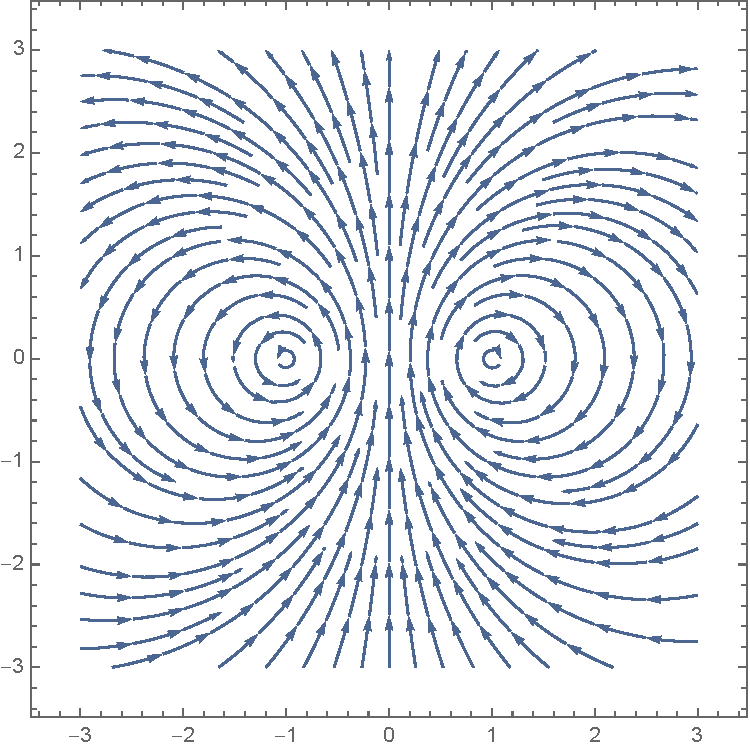
\includegraphics[width=100mm]{4_HW5.pdf}
		\end{figure}
	
	For the vector potential, we note that it must only have a component parallel/antiparallel to the current $I$, i.e. 
	\[
		\vect A = A \vecth z.
	\]
	Using $\vect B = \del\times \vect A$ and the Coulomb gauge $\del\cdot \vect A = 0$ we can deduce the following for $\vect A$:
	\[
		\pdiff[A]{y} = B_x,\quad \pdiff[A]{x} = -B_y,\quad \pdiff[A]{z} = 0.
	\]
	From the last relation we see that $A$ must be a function of $x$ and $y$ only. From the other two relations we have
	\[
		A = \frac{\mu_0 I}{2\pi} \int dy\, \plr{\frac{-y}{(x+a)^2+y^2}+\frac{y}{(x-a)^2+y^2}} + f(x)
	\]
	\[
		A = \frac{-\mu_0 I}{2\pi} \int dx\, \plr{\frac{x+a}{(x+a)^2+y^2}-\frac{x-a}{(x-a)^2+y^2}} + g(y).
	\]
	All these integrals have the same form
	\[
		\frac{1}{2} \ln\plr{u^2+a^2}.
	\]
	Evaluating them we have
	\[
		A = \frac{\mu_0 I}{4\pi}\clr{-\ln[(x+a)^2+y^2]+\ln[(x-a)^2+y^2]} + f(x)
	\]
	\[
		A = \frac{\mu_0 I}{4\pi}\clr{-\ln[(x+a)^2+y^2]+\ln[(x-a)^2+y^2]} + g(y) .
	\]
	We can see that a nice simple form for the vector potential that satisfies our requirements is
	\[
		A = \frac{\mu_0 I}{4\pi}\ln\blr{\frac{(x-a)^2+y^2}{(x+a)^2+y^2}}.
	\]
	In summary we have
	\ba
		\vect B(x,y) =& \frac{\mu_0 I}{2\pi}\Bigg[\plr{\frac{-y}{(x+a)^2+y^2}+\frac{y}{(x-a)^2+y^2}}\vecth x \\
		&\quad\quad+\plr{\frac{x+a}{(x+a)^2+y^2}-\frac{x-a}{(x-a)^2+y^2}}\vecth y\Bigg].
	\ea
	\[
		\vect A = \frac{\mu_0 I}{4\pi}\ln\blr{\frac{(x-a)^2+y^2}{(x+a)^2+y^2}}\vecth z.
	\]
	\\
% #5 ------------------------------------------------------------------------------------------------------------------------------------------------------------------------------------
	\item
	Find the vector potential $\vect A(\vect r)$ and magnetic induction $\vect B(\vect r)$ produced by a thin current ring of radius
	$a$. The current value is $I$. Express the results in terms of elliptic integrals (5.5 Jackson).
	\\
	\\
	First let us situate the ring of current of radius $a$ to lie in the $x$-$y$ plane and centered at the origin. To find the vector
	potential, we will need to use Jackon eq. 5.32
	\be\label{7}
		\vect A(\vect x) = \frac{\mu_0}{4\pi}\int \frac{\vect J(\vect x')}{|\vect x-\vect x'|}d^3x'.
	\ee
	As usual, $\vect A$ lies in the same direction as $\vect J$. For the current density, we use
	\be\label{8}
		\vect J = J\vecth \phi = I\sin\theta'\delta(\cos\theta')\frac{\delta(r'-a)}{a}\vecth \phi.
	\ee
	From this we can see that $\delta(r'-a)$ restricts the current to a ring of radius $a$ and $\delta(\cos\theta')$ places the ring at 
	the origin $\theta = \frac{\pi}{2}$. If we break up $\vect J$ into its cartesian components we have
	\be\label{9}
		\vect J = J\sin\phi' \vecth x + J\cos\phi' \vecth y 
	\ee
	where the magnitude $J$ is given by \eqref 8. Before we substitute \eqref 9 into \eqref 7 it would be beneficial to note some symmetries. 
	Since the current distribution is cylindrically symmetric, it would suffice to calculate the vector potential only within one plane, say
	the $x$-$z$ plane ($\phi' = 0$). In addition, we note that integration \eqref 7 over $d\phi'$ is symmetric about $\phi'=0$ and since 
	the $x$ component of $\vect J$ is an odd function it will vanish. Thus we only integrate over the $y$ component of $\vect J$ and 
	have
	\[
		A(r,\theta) = \frac{\mu_0 I}{4\pi a}\int r'^2\, dr'\, \sin\theta'\, d\theta'\,d\phi' 
		\frac{\sin\theta'\cos\phi'\delta(\cos\theta')\delta(r'-a)}{|\vect x-\vect x'|}.
	\]
	For the distance vector $r$ making a polar angle $\theta$, the law of cosines can be used to show that
	\[
		|\vect x-\vect x'| = [r^2+r'^2-2rr'(\cos\theta\cos\theta'+\sin\theta\sin\theta'\cos\phi')]^{1/2}
	\]
	in which the integral becomes
	\[
		A(r,\theta) = \frac{\mu_0 I}{4\pi a}\int r'^2\, dr'\, \sin\theta'\, d\theta'\,d\phi' 
		\frac{\sin\theta'\cos\phi'\delta(\cos\theta')\delta(r'-a)}{[r^2+r'^2-2rr'(\cos\theta\cos\theta'+\sin\theta\sin\theta'\cos\phi')]^{1/2}}.
	\]
	Evaluating the delta functions we then have
	\[
		A(r,\theta) = \frac{\mu_0 I a}{4\pi} \int_0^{2\pi} \frac{\cos\phi'\, d\phi'}{(a^2+r^2-2ar\sin\theta\cos\phi')^{1/2}}.
	\]
	This integral is an elliptic integral. It can be expressed in the form of complete elliptic integrals of the first and second kind respectively
	as
	\[
		K(k) = \int_0^{\pi/2} \frac{d\theta}{\sqrt{1-k^2\sin^2\theta}}
	\]
	and
	\[
		E(k) = \int_0^{\pi/2}d\theta\, \sqrt{1-k^2\sin^2\theta}.
	\]
	By expressing the parameter $k$ as
	\[
		k^2 = \frac{4ar\sin\theta}{a^2+r^2+2ar\sin\theta}
	\]
	the vector potential can be brought to the form
	\be\label{10}
		A(r,\theta) = \frac{\mu_0}{4\pi}\frac{4Ia}{\sqrt{a^2+r^2+2ar\sin\theta}}\blr{\frac{(2-k^2)K(k)-2E(k)}{k^2}}.
	\ee
	To find the magnetic field, we simply use $\vect B = \del\times \vect A$ to find
	\[
		\vect B = \frac{1}{r\sin\theta}\pdiff[]{\theta}(\sin\theta A)\vecth r -\frac{1}{r}\pdiff[]{r} (rA)\vecth\theta.
	\] 
	To find the magnetic field in a more explicit form in terms of elliptic integrals, we need to differentiate:
	\[
		B_r = \frac{1}{r\sin\theta}\cos\theta A+\frac{1}{r}\pdiff[A]{\theta}
	\]
	\[
		B_\theta = -\frac{A}{r}-\pdiff[A]{r}.
	\]
	The partial derivatives of $A$ are
	\ba
		\pdiff[A]{\theta} =& -\frac{\mu_0}{8\pi}\frac{8Ia^2r\cos\theta}{(a^2+r^2+2ar\sin\theta)^{3/2}}\blr{\frac{(2-k^2)K(k)-2E(k)}{k^2}}\\
		&\quad +  \frac{\mu_0}{4\pi}\frac{4Ia}{\sqrt{a^2+r^2+2ar\sin\theta}}\pdiff{\theta}\blr{\frac{(2-k^2)K(k)-2E(k)}{k^2}}
	\ea
	\ba
		\pdiff[A]{r} =& -\frac{\mu_0}{8\pi}\frac{4Ia(2r+2a\sin\theta}{(a^2+r^2+2ar\sin\theta)^{3/2}}\blr{\frac{(2-k^2)K(k)-2E(k)}{k^2}}\\
		&\quad +  \frac{\mu_0}{4\pi}\frac{4Ia}{\sqrt{a^2+r^2+2ar\sin\theta}}\pdiff{r}\blr{\frac{(2-k^2)K(k)-2E(k)}{k^2}}.
	\ea
	If we want, we could go further and very explicitly evaluate $\pdiff[k]{r}$, $\pdiff[k]{\theta}$, $\pdiff[K(k)]{r}$, $\pdiff[K(k)]{\theta}$, 
	$\pdiff[E(k)]{r}$, and $\pdiff[E(k)]{\theta}$ but this is quickly turning into a very lengthy exercise in partial derivatives. Therefore, 
	I shall leave here and express the magnetic field as
	\[
		\vect B =\plr{\frac{1}{r\sin\theta}\cos\theta A+\frac{1}{r}\pdiff[A]{\theta}}\vecth r -\plr{\frac{A}{r}-\pdiff[A]{r}}\vecth\theta.
	\] 
	where $\ds\pdiff[A]{r}$ and $\ds\pdiff[A]{\theta}$ are given in terms of elliptic integrals above and $A$ is given by \eqref{10} . 
		
\eenum
\end{document}